% !TeX root = ../main.tex

\chapter{绪论}

\section{研究背景与意义}
近年来,我国持续面临人口老龄化问题。根据《2021年度国家老龄事业发展公报》的数据\cite{2021NianDuGuoJiaLaoLingShiYeFaZhanGongBao},到2021年末,全国有60岁及以上的老年人口达到2.6亿,占总人口的18.9\%;65岁及以上的老年人口为2亿,占总人口的14.2\%,65岁及以上老年人口的抚养比为20.8\%。《中国养老服务蓝皮书(2012—2021)》\cite{YangZhongGuoYangLaoFuWuLanPiShu201220212022}显示,2015年我国失能和部分失能老人人数约为4063万,占老年人口的18.3\%。预计到2025年,失能老人人数将增至7279.22万,到2030年将达到1亿。目前,独居或空巢老人数量已达到1.18亿。多数情况下,由于子女与老人分居,老人主要获得的是经济支持,而非生活照料和情感陪伴等家庭式养老支持,这一状况严重影响了独居或失能老人的生活质量。因此,针对老年和残疾人群的康复辅助机器人的研发对于减轻社会养老压力、提高失能老人的独立生活能力和自信心具有极其重要的意义。

康复辅助机器人一般用于辅助或扩展人类的运动和/或认知能力,主要面向对象为:体弱的老人、截肢者和其他患有脊髓损伤、中风等疾病的人群。 近年来,我国先后颁布了《中国制造2025》\cite{ZhongGuoZhiZao2025}、《“健康中国2030”规划纲要》\cite{LiuYangJianKangZhongGuo2030GuiHuaGangYao}等文件,重点支持康复辅助机器人产业发展。辅助机器人一般需要其拥有智能化和鲁棒性以维持系统的安全高效性和灵活性,通过集成在线信息处理机制,机电一体化和先进的人机交互接口与人进行物理或者其他感官接触。尽管近年来机器人技术以及模式识别技术取得了巨大的进展,在辅助机器人领域,我们仍远未为机器人提供完全的自主权,从而使它们能够在动态变化的环境中能够处理更多的情况。

近年来,以机器学习和深度学习为代表的机器智能技术的快速发展并取得显著成果。然而,随着数据量增加,``智能提升''逐渐减弱。与此同时,人工智能系统与人类之间的互动关系变得更加广泛和复杂\cite{ZhaoQianTanKongZhiZhongDeGongXiangXinXiHeGongXiangZiZhu2021}。相较于人类智能,机器智能通常根据当前对外部环境的感知给出确定性的决策,灵活程度低且容易受到感知系统输入不确定性的影响导致决策失败。然而,机器决策在动态变化的环境下往往可以产生高维度的操控指令并作出最优的决策,进而保证系统的整体安全高效。然而,在大多数辅助机器人应用中,通常都由人类操作者操作或监督机器人。在康复辅助机器人系统中,使用者一般都存在显著认知和运动障碍,通常仅能使用有限离散的交互接口导致基于交互界面的人类决策输入存在更高程度的交互不确定性,容易造成意外情况出现。相较于机器智能,人类操作者能够提供优越的情境感知、逻辑和解决问题的能力,但这也提出了一个核心问题:在需要保证安全可靠性的人-辅助机器人交互系统中,我们应当怎样处理用户的交互输入的不确定性。

在物理人-机器人交互领域,机器自主是一种手段,而不是目标,自主级别因应用领域的不同存在差异。与智能控制器共享机器人系统的控制,可以让人类在执行任务时减少认知和身体上的工作量,在另一方面机器智能又能够在一定程度上纠正使用者的错误输入。在``通用人工智能''时代真正到来之前,人机混合将长期存在于辅助机器人系统中\cite{ZhangMianXiangRenJiXuGuanJueCeDeHunHeZhiNengFangFaYanJiu2021}。因此,如何在康复辅助机器人的交互系统设计中分析和动态处理人类输入的不确定性,对于提高康复辅助机器人系统的个体适应性和安全性,减轻使用者负担,促进相关技术应用落地具有重要意义。

\section{康复辅助机器人研究现状}
康复辅助机器人技术旨在为残疾患者提供支持,使他们能够更独立地进行日常生活活动(Activities of Daily Life, ADL)。例如,移动、抓握和处理物体、进食等。目前该领域的研究涉及机械,信息,控制,计算机,医学等多个学科,是当前机器人研究领域的热点。目前的辅助设备如电动轮椅、辅助机械臂、上肢或下肢外骨骼机器人和主动矫形器,对于帮助那些有严重运动障碍的人改善独立生活能力、减轻家庭照护负担至关重要。

在图\ref{fig:1-1}中给出了康复辅助设备在助老助残领域不同阶段中的典型应用需求场景。在损伤的早期阶段,轮椅以及其他移动辅助设备主要服务于那些没有或几乎没有自主移动能力的个体。随着康复进程的深入,特别是到了中期阶段,个体的自主移动能力得到了一定程度的恢复和改善,这时他们对于辅助设备在进行坐到站等身体状态转变中的帮助需求变得更加迫切和明显。至于康复的后期阶段,助力使用者恢复独立行走和其他自主日常活动能力,则成为康复辅助机器人设计和开发的主要目标。在使用者与移动辅助设备的交互中,交互感知系统通常仅需捕获使用者可产生的局部动作产生交互命令,例如操纵杆、开关控制器、面部识别等。在与状态转移辅助设备的交互中,智能化的辅助设备对交互感知系统提出了更高的要求,通常需要获取被辅助对象更加全面的交互信息,例如身体姿态、接触力等。该类型的运动时间通常较短,且开始和结束时的速度一般为零,因此在交互过程中更需要考虑个体适应性问题。步行运动辅助是最为复杂的交互场景,不同于状态转移辅助通常为一个点到点的运动任务,步行运动的持续时间通常更长,且是一个连续的周期运动。因此,在步行辅助机器人的交互中,不仅仅需要考虑到由于步态特征以及康复阶段不同导致的个体适应性问题,系统安全性问题也同样重要。

\textbf{尽管在不同应用场景中三种康复辅助机器人的设计目标不同,但是其中的人机交互问题是相通的,均包含了运动感知、意图推理等共性问题}。因此,本节首先对这三种类型的康复辅助机器人的相关研究进行了介绍和总结,并在后续的内容中对其中的共性交互感知方式进行了分析。

\begin{figure}[htb]
  \centering
  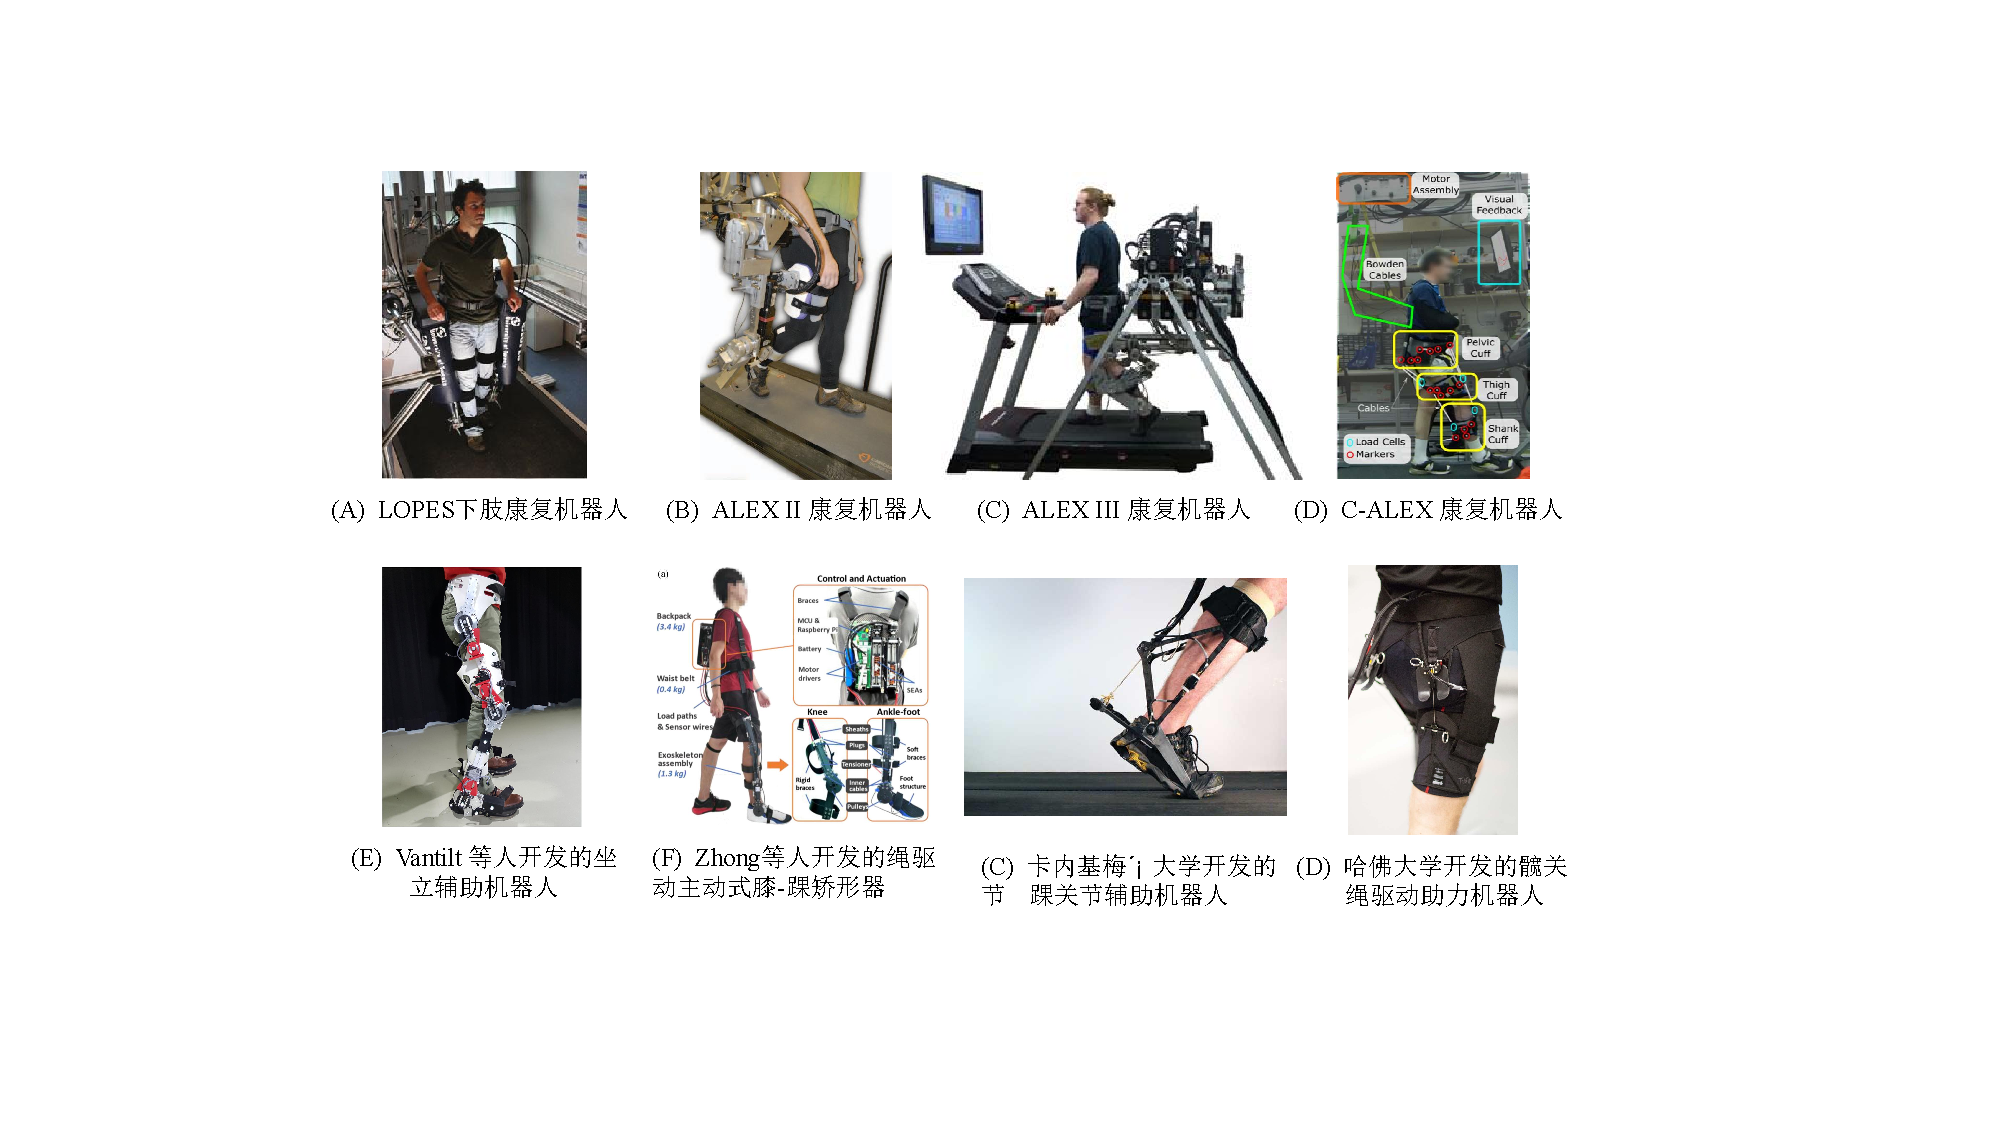
\includegraphics[width=0.9\textwidth]{1-Fig-1.pdf}
  \caption{康复辅助设备在助老助残领域中的典型应用需求场景}
  \label{fig:1-1}
  % \note{Exoskeleton robots developed by some universities and companies}
\end{figure}

\subsection{移动辅助机器人}
相对于可穿戴式辅助机器人用于移动支持,轮椅是最常用的辅助设备\cite{worldhealthorganizationGuidelinesProvisionManual2008b}。根据国家卫健委和中国残疾人联合会公布的数据,我国失能、半失能老年人口高达4200万人,肢体残疾人人数约为2472万人,预计轮椅的实际需求用户接近4000万人。那些由于认知、运动或感觉障碍而受影响的个体,无论是由于残疾还是疾病,通常依赖于电动轮椅来完成移动任务。为了满足那些在操纵传统轮椅方面面临困难或无法操纵的个体的需求,一些研究人员已经引入最初用于移动机器人的技术,从而研发出智能轮椅。此外,由于一些残疾人无法使用传统的操纵杆来导航,因此需要采用替代的控制系统,如头部操纵杆、下巴操纵杆、抽吸器以及脑控技术\cite{kimLiteratureReviewSmart2023,carringtonWearablesChairablesInclusive2014,rulikControlWheelchairMounted6DOF2022}。这类移动辅助设备通常具有简单而易于操作的结构,不仅在为失能用户提供身体活动方面发挥着关键作用,同时也显著提升了他们的社会参与能力。目前,国际上研发智能轮椅的主要企业有 Permobil、Lucy Mobility 等,国内也有相关企业开始布局该领域,如椅夫健康、邦邦机器人,图\ref{fig:1-2}展示了部分国内外商业智能移动辅助机器人。这些企业在技术研发、产品创新和市场推广方面展现出强大的实力。目前,轮椅行业的技术正在升级,未来市场将以智能化、人性化为主流。此外,相关政策也提出支持改善老年人和残疾人的辅助用品适用性,要求针对特殊人群的消费品发展需求,加强人体工效学基础研究、技术开发和标准制定。

智能轮椅本质上为一个带有一系列如激光雷达、摄像头、红外线传感器等传感器和计算机控制系统的移动差速机器人\cite{ngIndirectControlAutonomous2020a,leamanComprehensiveReviewSmart2017},其智能体现在感知和操控两个方面\cite{kimLiteratureReviewSmart2023}。首先,在感知方面,是以自动避障,自动导航以及地形自适应等功能为代表的安全导航功能。近些年来,自动驾驶汽车领域学术和工业研究的爆炸式增长,使得自动驾驶技术在各个方面取得了显著进步,并被广泛应用于提升辅助轮椅的自动化水平。这一方面比较代表性的研究有MIT-CSAIL实验室研发的自主移动轮椅项目\cite{walterFrameworkLearningSemantic2014},其通过环境感知和无线室内定位系统开发了一款可以使用语音命令操控的自动导航轮椅,从而增强普通电动轮椅的功能。美国密歇根大学安娜堡Vulcan等人\cite{fosterReflectanceFieldMap2023,parkDiscretetimeDynamicModeling2017}开发的智能轮椅采用了一种混合空间语义层次结构算法用于进行导航空间知识表示,其能够实现高效学习和自然的人机交互。新加坡国立大学开发的全自动驾驶助行车\cite{SelfdrivingScooterUnveiled}可以用于在大型车辆难以通行的较小和较窄的道路上行驶。iBOT智能轮椅设计了四轮驱动底盘\cite{MobiusMobilityNext},利用地形跟踪技术实现了陡坡和各种地形的自适应,其座椅角度可根据坡度自动调节进而令使用者保持稳定。
\begin{figure}[h]
  \centering
  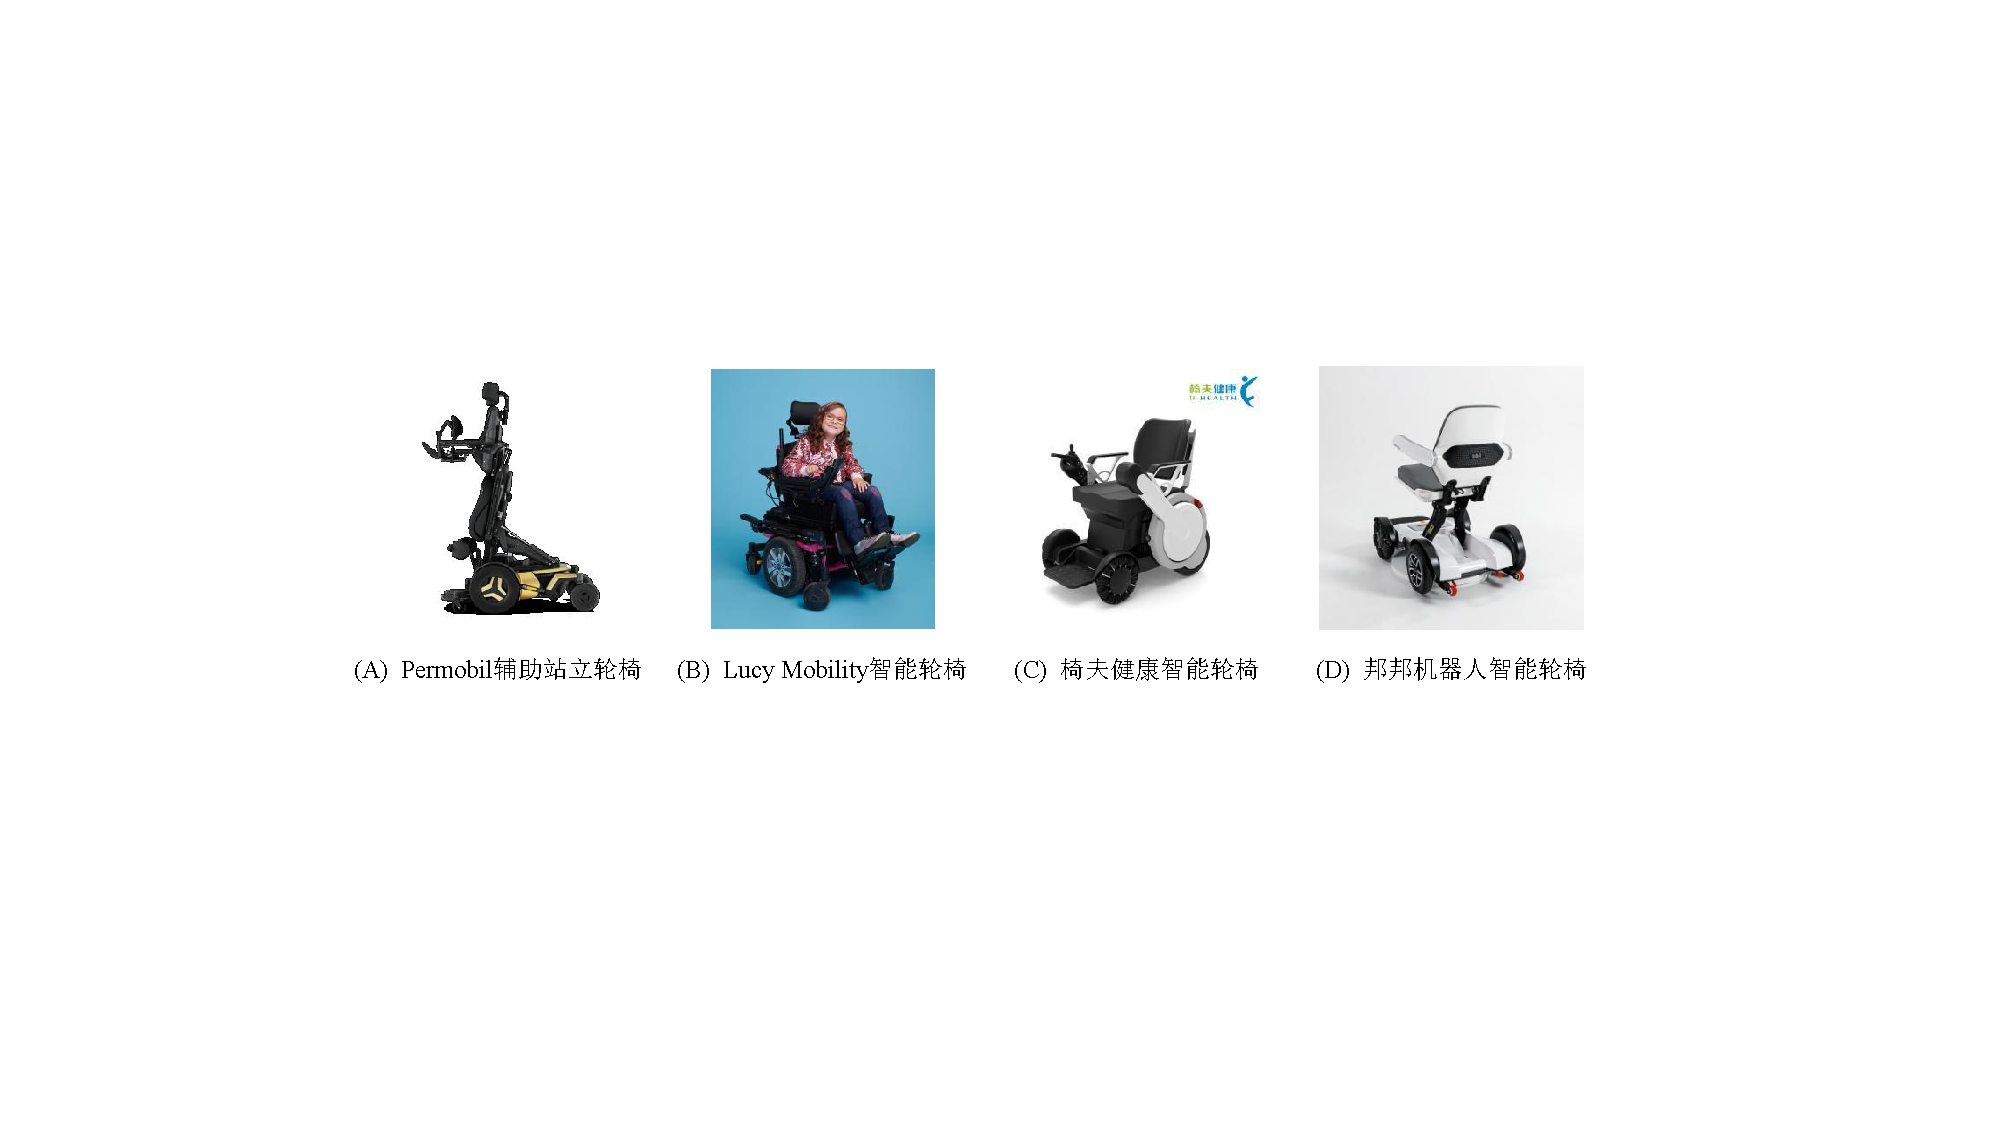
\includegraphics[width=1\textwidth]{1-Fig-2.pdf}
  \caption{国内外商业公司研发智能移动辅助机器人}
  \label{fig:1-2}
  % \note{Exoskeleton robots developed by some universities and companies}
\end{figure}

智能轮椅不仅要能感知世界、表达所学知识、做出有用的推断和计划,还必须能够与其他智能体,特别是与人进行有效的交流。由于缺乏运动能力、力量或存在视觉障碍,大量的使用者很难独立操作轮椅\cite{hartmanHumanMachineInterfaceSmart2019},因此在交互操控智能方面主要的工作是各种替代性的人机接口,以增加用户对移动辅助设备控制的自主权。对于患有运动神经元疾病(如肌萎缩侧索硬化症)的人群,脑机接口(Brain-Computer Interface, BCI)是目前最有应用潜力的研究方向之一。脑电图(Electroencephalogram, EEG)是BCI中使用的主要非侵入性技术之一,在图\ref{fig:1-3}(A)中给出了BCI操控电动轮椅的主要技术路线\cite{naserPracticalBCIDrivenWheelchairs2023}。其中,P300和SSVEP是两种最常用于识别用户的意图的BCI范式。P300范式依赖于检测用户大脑中的P300电位\cite{rebsamenBrainControlledWheelchair2010},而SSVEP范式依赖于检测用户大脑中的视觉诱发电位\cite{dongMultimodalBrainComputer2022,ngIndirectControlAutonomous2020a,mistrySSVEPBasedBrain2018}。

然而,基于EEG信号的人机界面通常存在带宽较低、学习周期长、计算要求高以及需要用户高度集中注意力等问题。此外,它们大多只能在有限的离散指令空间内工作。最近,有用户研究显示,瘫痪患者普遍表示更喜欢将人机界面嵌入可穿戴设备中\cite{zhangUnderstandingInteractionsSmart2022}。围绕这一问题,美国西北大学的Thorp等人\cite{thorpUpperBodyBasedPower2016d}针对四肢瘫痪患者设计了一种基于身体-机器接口(Body-Machine Interface, BoMI)的轮椅控制界面,通过放置在肩部的几个反光标记点以及光学相机,该系统可以允许使用者通过高维肩关节运动变化生成轮椅控制命令,进而提高用户操作的灵活性。随后Seáñez-González等人\cite{seanez-gonzalezStaticDynamicDecoding2017}在此基础进一步设计了一套基于惯性传感器网络的体-机交互设备,并深入地分析了不同数据映射方式在虚拟电动轮椅操控效果上的表现。此外,在反馈交互增强方面,Devigne等人\cite{devigneDesignHapticGuidance2018}设计了一套低复杂度优化框架的触觉反馈电动轮椅导航解决方案,通过向轮椅操纵杆发送力反馈来提供导航避障信息,以帮助轮椅用户更好地理解周围环境。Schettino等人\cite{schettinoImprovingGeneralisationLearning2020}基于一个力反馈控制器提出了一种学习辅助驾驶策略,通过使用自动编码器和高斯过程等模型来学习示教辅助策略以帮助轮椅使用者在空间中更好移动。

\begin{figure}[h]
  \centering
  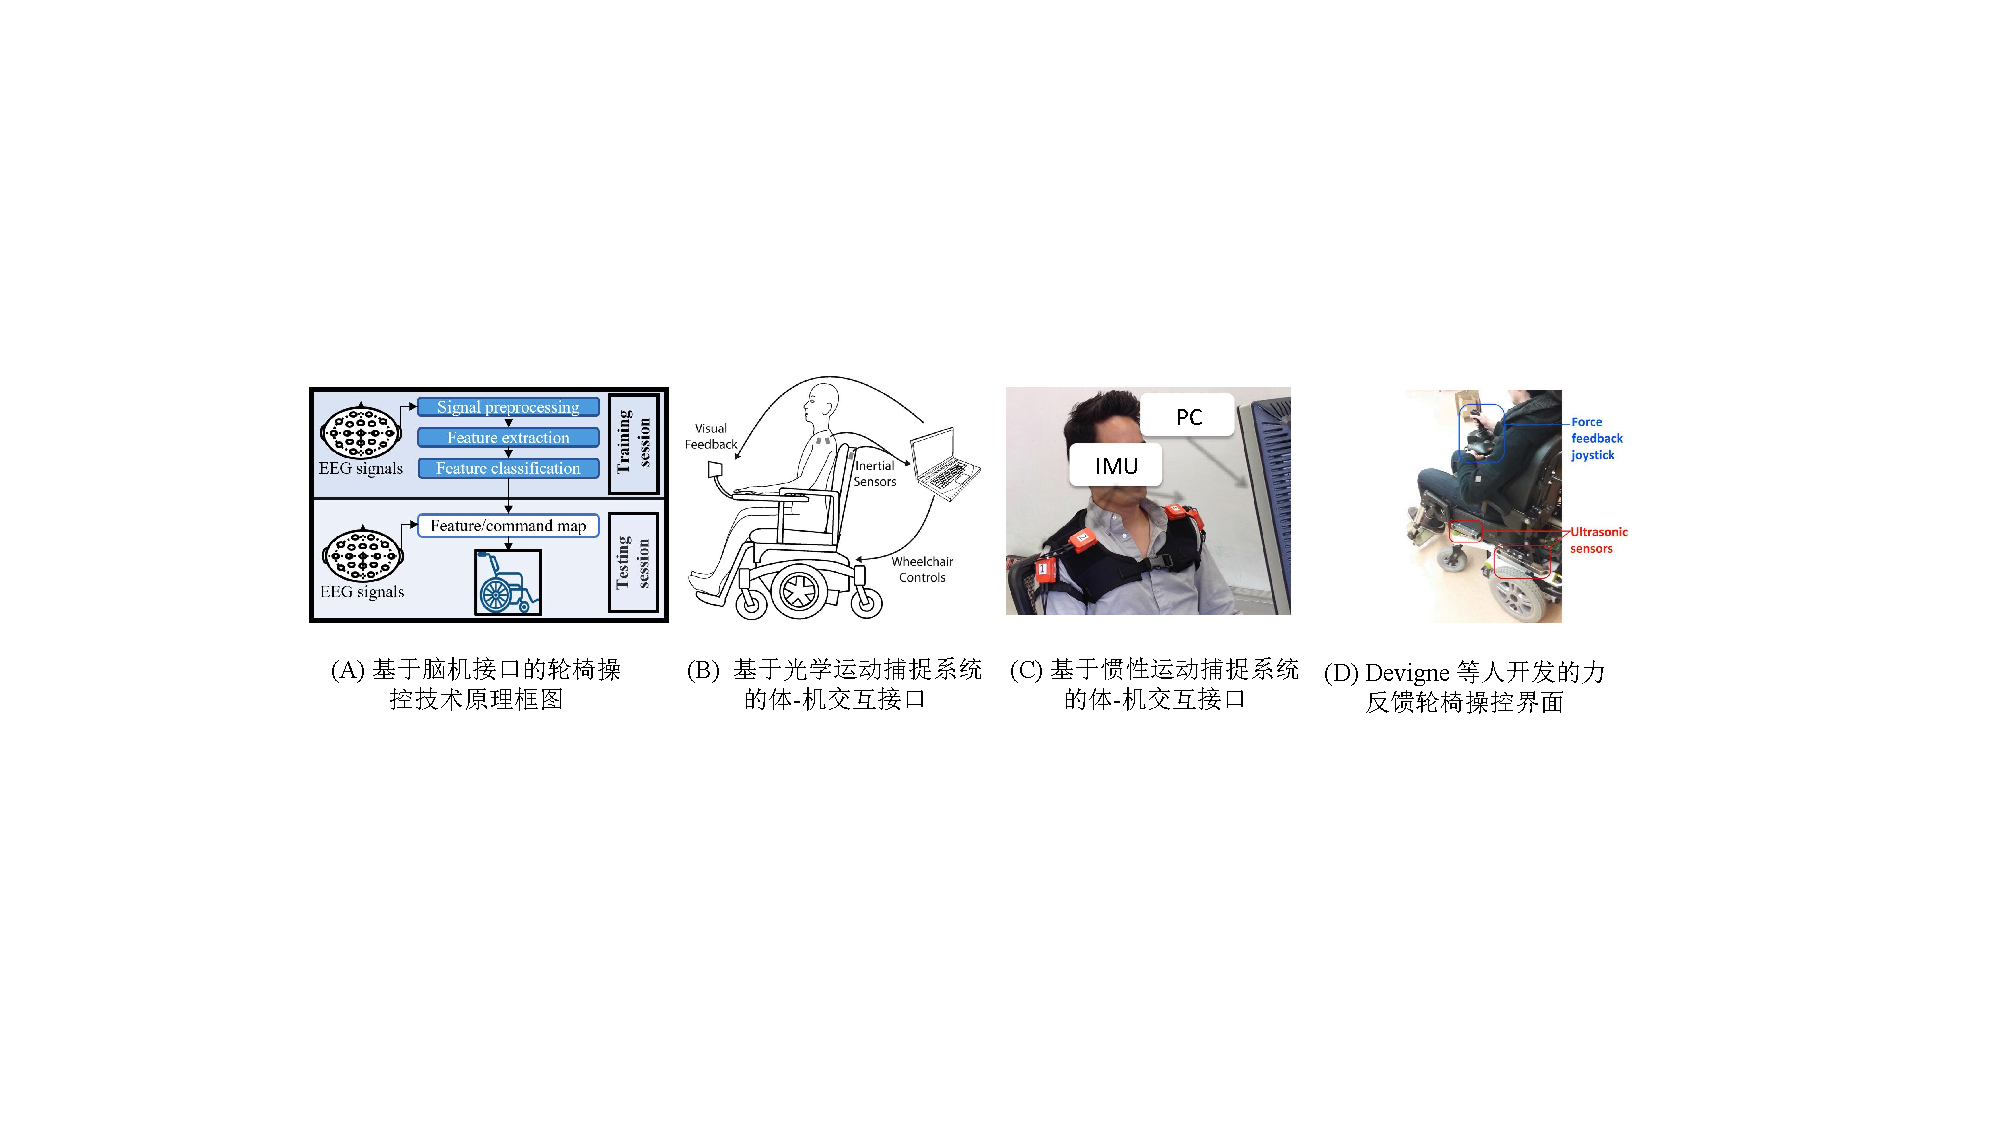
\includegraphics[width=1\textwidth]{1-Fig-3.pdf}
  \caption{智能轮椅操控界面相关研究成果}
  \label{fig:1-3}
  % \note{Exoskeleton robots developed by some universities and companies}
\end{figure}

\subsection{功能性辅助机器人}
人类由坐到站的转移(Sit-to-Stand, STS)是一种经常进行的日常活动,其中由于肌肉无力、关节病变、神经系统问题以及骨密度降低导致无法完成正常STS转移在高龄老人中普遍存在,这一问题对老年人的生活自理能力和生活质量产生了显著影响。除了为截瘫患者开发的全下肢外骨骼系统外,当前仅为支持人体由坐到站转移而专门设计的辅助机器人设备和相关研究并不是很多。与外骨骼式康复机器人类似,这些设备和被辅助的对象的交互控制机制可划分为三个主要类别,即开关控制、位置运动控制和力控制。其中开关控制普遍用在简单的辅助设备中,在本文不做讨论,接下来主要其余两种交互控制方式。

Jun和Kim等人\cite{hong-guljunWalkingSittostandSupport2011,inhokimKinematicAnalysisSittostand2011}开发了一个名为SMW的机器人,该系统主要基于一个支撑板辅助上身运动,并通过控制一个线性执行器跟随一个预定义轨迹来引导使用者由坐姿到站姿的转移。作者提出了两种预定义的轨迹,并利用位于支撑板的力和扭矩传感数据比较了它们的特性。Mederic和Pasqui等人\cite{medericElderlyPeopleSit2006}采用了力控制进行STS辅助,他们针对零力矩点的平衡约束最小化优化问题设计了一个简化的人体模型的零力矩点,并控制了用户和机器人之间的交互力。研究和模仿人类在进行STS转移时的行为,为控制辅助机器人以实现人类与机器人耦合系统的直观和自然行为提供了有力工具。其中人体STS转移过程中的下肢关节的扭矩和活动范围等运动学与动力学转移特征被广泛研究,例如Lindemann等人\cite{galliQuantitativeAnalysisSit2008}研究了正常STS期间下肢关节的扭矩和活动范围,Yoshioka等人\cite{yoshiokaBiomechanicalAnalysisRelation2009}通过研究大量实验收集的运动数据来确定最小峰值关节力和它们与运动时间的关系。

\begin{figure}[h]
  \centering
  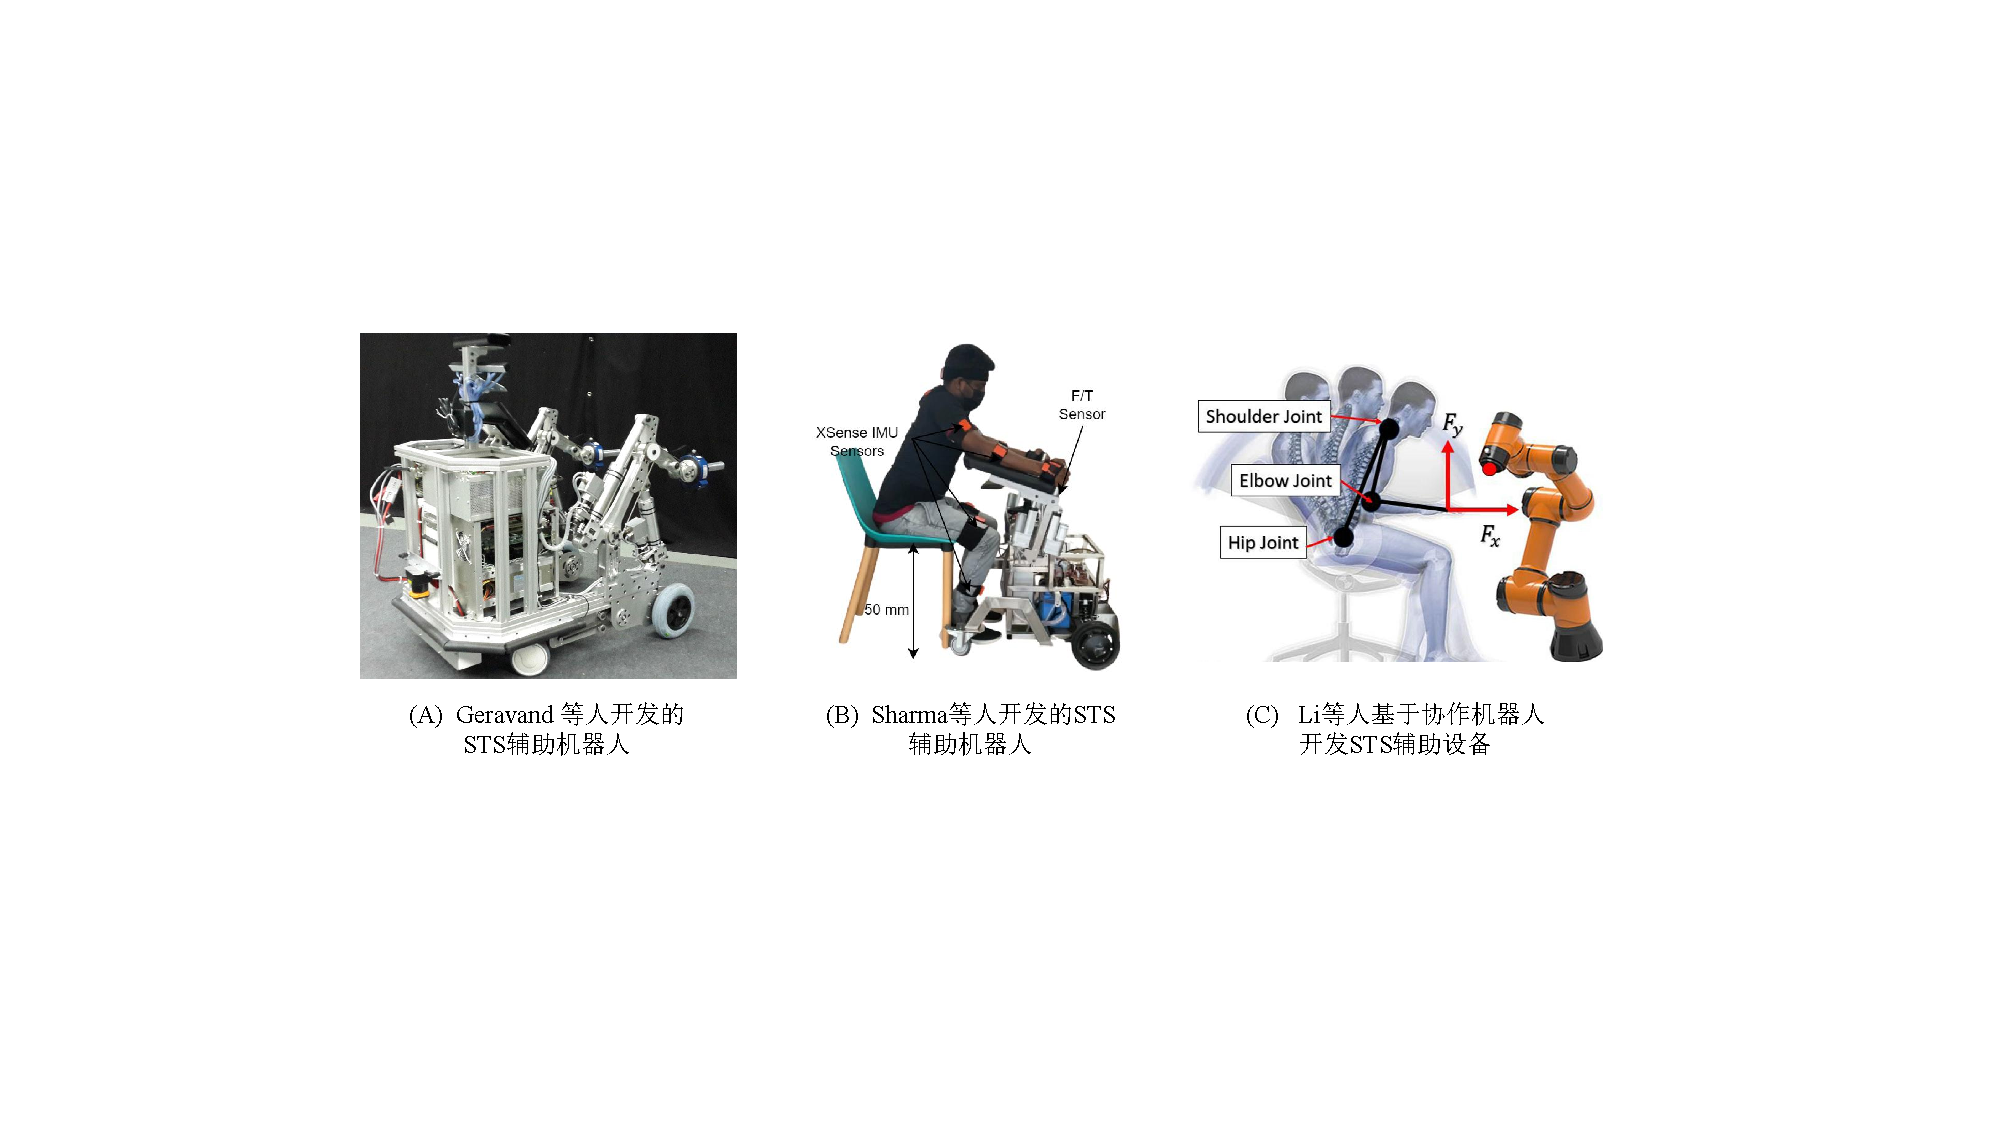
\includegraphics[width=1\textwidth]{1-Fig-4.pdf}
  \caption{智能站立辅助机器人的部分研究成果}
  \label{fig:1-4}
  % \note{Exoskeleton robots developed by some universities and companies}
\end{figure}

然而,以往关于人类STS转移辅助的研究很少结合STS转移运动的计算模型。大部分的研究主要集中在探索性和假设驱动的实验中进行研究与分析,从而得出了大量的研究成果。近年来,结合了人机耦合最优控制、骨骼肌肉模型、在线运动意图预测的交互式STS辅助设备成为研究主流,例如Geravand等人\cite{geravandHumanSittostandTransfer2017}基于一个STS辅助机器人提出了一种基于最优反馈控制的方法。该方法通过动态规划解决了一个优化问题,并推导出了最优的辅助策略,以提供由辅助机器人提供的辅助。此外,研究还通过实验验证了该方法的有效性,并评估了该方法对不同年龄和性别的老年人的适用性。Sharma等人\cite{sharmaBiomechanicalTrajectoryOptimization2022,sharmaPhysicalHumanRobotInteraction2022}提出了一种基于单位四元数动态运动基元(Dynamic Movement Primitives, DMP)的生物力学轨迹优化方法,用于分析人类STS运动。该方法结合了直接数值积分和概率路径积分(PI²)学习,以实现对生物力学系统的高效优化。Li等人\cite{liIntegratedApproachRobotic2021,liHumanCenteredControlFramework2018}提出了一种基于机器人辅助的坐立辅助方法,通过人机耦合动力学建模、人体关节控制机制和人类意图识别,实现了机器人辅助下的最优坐立辅助。该方法通过LSTM网络预测人类意图,并生成最优的机器人末端轨迹,从而优化了人体关节的负荷。Zuo等人\cite{zuoOnlineMonitoringHuman2023}提出了一种基于Karush-Kuhn-Tucker优化(KKT-ZSMF)的在线人类坐立运动监测算法。该算法通过动态稳定性区域建模和优化问题求解,实现了对老年人坐立运动稳定性的实时预测。实验结果表明,KKT-ZSMF算法在预测准确性和运行时间方面均优于其他算法,为STS过程中老年人的跌倒预防提供了有效的技术支持。此外,一些研究进一步从人体生物动力学的角度分析了人体STS过程的辅助策略,该类型的方法通过精确计算骨骼肌肉模型中的肌肉协同激活效应,可以帮助我们实现对肌肉激活能力的模拟仿真,从而实现对特定失能人群的模拟仿真。其中,Kumar等人\cite{kumarPredictingSittoStandAdaptations2022}提出了一种STS预测模型,通过优化算法生成了不同强度缺陷模型下的坐立轨迹,并分析了肌肉激活、肌肉力量和关节扭矩之间的关系。Gordon等人\cite{gordonLearningPersonalisedHuman2023a}通过收集4名受试者的坐立数据,提出了一种基于逆肌肉骨骼模型最优控制框架,用于学习人类STS运动的个性化辅助模型。

\subsection{关节运动辅助机器人}
关节运动辅助机器人的主要代表为主动矫形器与外骨骼机器人,经过数代发展,研究涌现出多种拥有不同驱动方式和控制方法的系统。其中物理人机交互控制系统是其核心部分,需要系统能够实时感知用户的运动意图和姿态,并根据这些信息控制机器人的动作,常用的控制方法包括基于模型的控制、基于传感器的控制和混合控制等。目前,相关研究更加强调在多学科领域的整合,包括生物力学、机器人工程、神经科学等多个学科的交叉,推动了该领域的不断创新。相较于外骨骼机器人,主动式矫形器和智能假肢主要用于帮助患者恢复行走能力,改善步态,减轻关节负担等,通常采用被动式或半主动式驱动方式,即根据患者的步态自动调整其支撑力和运动模式。而下肢外骨骼机器人则采用全主动式驱动方式,可以根据患者的需求和外部指令进行精确的运动控制,并用于康复训练、提高运动能力、增强体力等。

相对于需要携带自己的电池和执行器的完整外骨骼来说,主动矫形器作为一种靶向型外骨骼机器人普遍都有更低质量和转动惯量,因此驱动器的输出功率可以更多用于为用户提供辅助而不是补偿自身重量\cite{collinsReducingEnergyCost2015,zhangHumanintheloopOptimizationExoskeleton2017a}。其一般多为单关节结构,在保留使用者一部分自由活动能力的前提下通过驱动器辅助特定关节来完成运动动作,其可分为髋关节、膝关节或踝关节辅助系统\cite{malcolmExperimentalStudyRole2009}。在步行中,膝关节主要是一个自由阻尼关节,在摆动阶段几乎处于锁定状态,而在支撑阶段则与之相反;髋关节和踝关节主要与摆动阶段的动态处理和支撑阶段的地面推进有关。目前主动式矫形器的控制方式主要有基于自适应振荡器的控制、基于模型的控制、基于预定义步态模式动作以及基于强化学习与在线优化等四种方式\cite{yanReviewAssistiveStrategies2015}。

图\ref{fig:1-5}展示了部分高校和公司研发的外骨骼式辅助机器人。Ronsse等人\cite{ronsseOscillatorbasedAssistanceCyclical2011c}开发的LOPES机器人最先使用了自适应非线性振荡器实现了髋、膝关节辅助。它通过利用自适应振荡器池来提取髋关节角度的相位和频率,再将这些相位及髋关节角度信息输入到核心滤波器中,实现对髋关节角度的无延迟估计。然后,计算出所需的关节扭矩,以便驱动髋关节移动至预测的下一个位置。此外,与LOPES机器人类似,ALEX系列机器人\cite{winfreeDesignMinimallyConstraining2011,stegallVariableDampingForce2017,hidayahGaitAdaptationUsing2020}也基于髋关节的运动特征实现了在线步态分析并为使用者施加髋关节辅助扭矩。基于模型的控制方式主要有赖于建立人机耦合物理模型来确定执行器的输出。在人形机器人领域,基于模型的控制系统策略通常需要充分考虑完整的机器人动力学。然而,在辅助机器人领域,模型有所不同,主要区别在于系统中引入了人类。其中,一个关键因素是对人与环境之间的接触进行建模\cite{youngStateArtFuture2017a}。 基于一个单自由度下肢辅助机器人,Aguirre-Ollinger等人\cite{aguirre-ollingerInertiaCompensationControl2012}提出了一种人体-外骨骼导纳控制模型,其生成的参考轨迹通过一个由线性二次型调节器(Linear Quadratic Regulator, LQR)和积分项组成的闭环控制器进行跟踪。通过将外骨骼机器人的动力学模型分解为摆动相和支撑相,王立坤等人\cite{WangXiaZhiZhuLiWaiGuGeJiQiRenKongZhiXiTongRenJiGongRongCeLueYanJiu2019}提出一种基于混杂自动机的下肢助力外骨骼机器人动力学系统。为了实现一个基于串联弹性单元驱动的外骨骼动力学补偿和用户特定的辅助,Vantilt等人\cite{vantiltModelbasedControlExoskeletons2019}通过对完整的外骨骼动力学和与环境接触的建模,实现了用户由坐到站的辅助。

\begin{figure}[h]
  \centering
  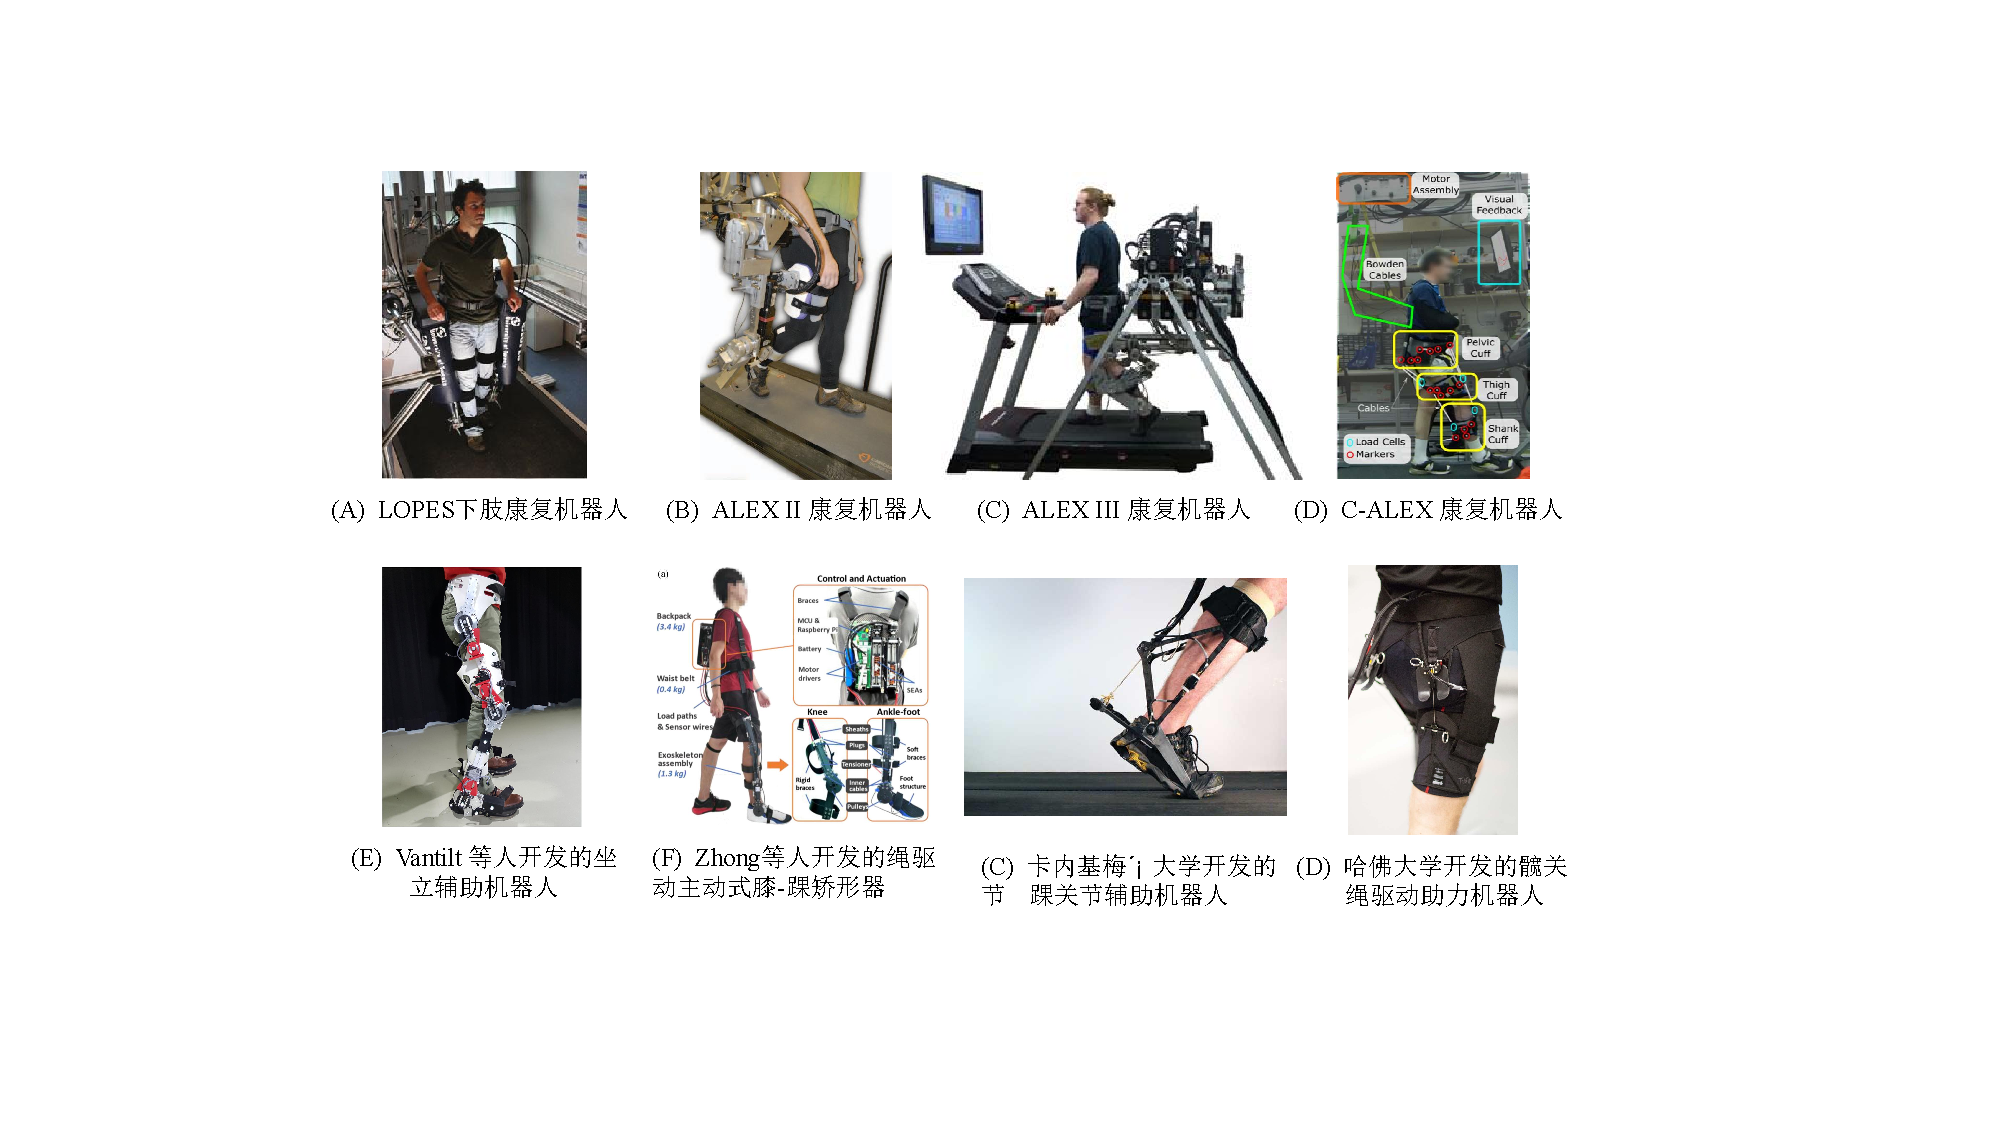
\includegraphics[width=1\textwidth]{1-Fig-5.pdf}
  \caption{部分高校和公司研发的主动矫形器与外骨骼式关节运动辅助机器人}
  \label{fig:1-5}
  % \note{Exoskeleton robots developed by some universities and companies}
\end{figure}

建立精确的人机耦合动力学模型往往较为困难,预定义轨迹由于实现较为简单,是目前商业应用中最常见的模式。基于预定义轨迹的控制器通常用于步态训练器和完全截瘫患者的外骨骼,并通过位置或阻抗控制来实现轨迹跟随。预定义参考轨迹通常来自健康人群的运动数据或者直接通过人工设置,但是其通常无法实现使用者的个性化运动模式。例如Zhong等人\cite{zhongGaitSymmetryEnhancement2022}采用预定义力矩辅助曲线和一个基于串联弹性单元驱动器的膝-踝-足矫形器实现了下肢步行辅助。近年来,由于系统允许佩戴者自由地在无约束环境下进行移动,围绕单关节靶向式外骨骼设备,基于在线学习与优化方式的控制器逐渐成为主流研究方向。Kawamoto等人\cite{kawamotoModificationHemiplegicCompensatory2015,kawamotoDevelopmentAssistController2014a}设计了一个单腿版本的混合辅助肢体(Hybrid Assistive Limb, HAL),在摆动阶段为受影响的肢体提供帮助,其中使用一个运动缓存器来在线存储未受影响肢体的运动数据用规划机器人运动轨迹。Huang和Peng等人\cite{huangLearningbasedWalkingAssistance2018,pengDataDrivenReinforcementLearning2020}提出了一种基于强化学习的步行辅助控制策略。他们通过将未受影响的一方作为领导者,将外骨骼作为追随者来模拟机器人控制系统。相较于简单的预定义轨迹,人在环中优化算法可以实时为参与者个性化辅助机器人控制参数,避免了需要对人机耦合系统进行精确建模这一技术难点,为辅助机器人个性化提供了可能。卡内基梅隆大学和哈佛大学\cite{dingHumanintheloopOptimizationHip2018,zhangHumanintheloopOptimizationExoskeleton2017a,awadSoftRoboticExosuit2017}所开发的一系列绳驱动柔性外骨骼系统已证明使用辅助髋部和踝关节运动的外部设备可减少使用者在步行时的代谢消耗。

\section{人-机器人交互感知系统研究现状}
人-机器人交互感知目前是一个极为多元化的研究领域,主要聚焦于理解、设计和评估机器人系统,以供人类使用,或与人类进行物理接触或远程操控。从本质上而言,人-机器人交互感知系统的问题在于通过评估双方的能力和设计,形成适当的互动技术,以理解和塑造人类与机器人之间的互动。这使得该领域成为了一个需要结合多学科知识进行研究的领域,例如神经科学、计算机科学、心理学、认知科学、医学以及工业设计等\cite{mohebbiHumanRobotInteractionRehabilitation2020a}。人与机器人之间的交互具有多种模式。大体上,这些模式可以划分为两类关系:\textbf{平行关系}和\textbf{层级关系}\cite{liuDesigningRobotBehavior}。

在平行关系中,人和机器人被视为相互独立的智能体。它们之间不存在显著的主从关系,各自根据自己的认知能力做出决策。这种关系下常见的交互情景例子有处于自动驾驶状态的汽车和人类驾驶的汽车或行人、人类和协作机械臂等。他们之间的角色划分可以为相互协作去完成一个共同的目标,也可以是竞争和博弈去使得自身的利益最大化。在这种交互模式中人类和机器人一般不存在直接的物理接触,因此在机器人端的感知系统的设计中一般都使用非侵入式的视觉、雷达、红外等环境感知传感器。从算法设计的角度,针对平行结构的人-机器人交互的研究大多从笛卡尔空间中的多智能体博弈的角度展开。此外,由于人和机器人系统往往都无法获得对环境以及对方状态全部信息,因此意图推理\cite{fangBehavioralIntentionPrediction2023}以及意图可视化\cite{szafirConnectingHumanRobotInteraction2021}用于是目前重要的研究方向。

在层级关系中,人和机器人之间存在比较明显的主从性,其中一方需要将一部分决策权让渡给另一方,服务机器人大部分工作在这种关系中。其中常见的交互情景例子有驾驶员和开启了辅助驾驶功能的智能汽车、人和遥操作机器人或手术机器人以及本文的主要研究对象人和康复辅助机器人等。不同于平行关系,人和机器人在层级关系中的角色划分更多的是协作,这主要是因为人类和机器各自具有独特的优势,其中人类具有更强的主观意识、判断力和决策能力,并且能够考虑伦理、道德、情感等因素,对任务进行整体把握。相反,机器人具有更为强大的计算能力和数据处理能力,且可自动化执行重复性、繁琐甚至危险的任务。然而,在动态变化的外部环境中,机器人和人类对于环境状态的处理能力通常是时变的(例如,在正常安全情况下,辅助驾驶系统负责做出决策;在紧急情况下,则要求人类接管)。而在辅助机器人系统的开发中,由于被辅助对象可能残疾、患有疾病或有其他身体障碍,机器人需要具有对被辅助对象在关节空间,甚至更深层次结构(例如神经、肌肉)的态势感知能力。

围绕康复辅助机器人的人体运动学估计,存在大量基于不同类型传感器以及数据处理方法的研究工作。感知系统的结构复杂度由低到高大致可以分为基于物理机械信号、基于可穿戴设备运动跟踪、基于视觉或语言的非侵入式感知、基于生理电信号以及多模态方法等几种类型。表\ref{tab:Sensors}对比了目前这几种常用技术路线的特点。其中基于物理机械信号的交互感知手段由于其结构简单、可靠性高,目前在各种类型的电动康复辅具上使用得最为广泛。其中压力传感器、扭矩传感器、振动或杠杆开关等大多应用于功能性的护理机器人当中。例如,通过压力传感器可以感知用户身体的压力分布,从而判断用户是否处于正确的姿势\cite{sharmaPhysicalHumanRobotInteraction2022};扭矩传感器可以感知用户施加的关节力矩,从而实现力度的调节和控制\cite{chenDevelopmentWearableUpper2022};振动或杠杆开关则可以通过用户的振动或位移来实现一些简单功能的触发。
\begin{table}[htb]
  \centering
  \caption{康复辅助机器人中常用的人机交互感知技术手段}
  \label{tab:Sensors}
  \begin{tabular}{cp{2.5cm}p{2.7cm}p{2.4cm}p{2.4cm}}
    \toprule
    \textbf{类型} & \textbf{感知方式} & \textbf{优势} & \textbf{缺点} & \textbf{主要应用领域}  \\
    \midrule
    \multirow{3}*{基于机械信号} & 压力传感器 & 精确检测压力大小和分布,实时调整辅助设备 & 维护和校准复杂、响应速度较慢 &  移动辅助机器人、假肢、辅助站立机器人\\
    ~ & 单/多维力传感器 & 上肢康复机器人、下肢康复机器人、外骨骼机器人 & 成本较高,且需要标定 & 站立辅助机器人、协作机器人 \\
    ~ & 触控、物理开关 & 上肢康复机器人、下肢康复机器人、外骨骼机器人 & 主要为开关量,感知能力单一 & 外骨骼机器人、移动辅助机器人 \\

    \multirow{3}*{\shortstack{基于可穿戴设备\\进行运动跟踪}}  & 舌动、牙齿触碰信号 & 适用于严重失能人群 & 存在卫生问题、影响使用者语言功能 & 移动辅助机器人、计算机控制 \\
    ~ & 惯性传感器 & 快速响应,实时性好,适用于一般动作跟踪 & 存在积分漂移问题、容易受到外部扰动 & 外骨骼机器人、虚拟现实、移动辅助机器人\\
    ~ & 柔性传感器、电子皮肤 & 无创、侵入性低、稳定性高且不易受外界干扰 & 成本较高、存在材料选择与制造工艺等技术难点 & 人形机器人、外骨骼机器人\\

    \multirow{2}*{\shortstack{非侵入式感知}}  & 视觉感知 & 测量范围广,响应速度快 & 易受光照等外部因素影响 & 移动辅助机器人、外骨骼机器人 \\
    ~ & 语音交互 & 侵入性低、交互信息丰富 & 无法实现实时交互、易受噪音影响 &  聊天机器人、生活辅助机器人、智能轮椅系统 \\

    \multirow{3}*{基于生理电信号} & 脑电图(EEG) & 具有开发神经假体的潜力,可实现高级别的意图识别 & 信噪比低,侵入性较强 & 移动辅助机器人、假肢、辅助机械臂、外骨骼机器人 \\
    ~ & 眼电图(EOG) & 技术较为成熟 & 舒适性和便携性差 & 移动辅助机器人、虚拟现实、计算机控制 \\
    ~ & 肌电图(EMG) & 高时间分辨率,能准确反映肌肉活动状态,抗干扰能力强 & 需要控制肌肉力量,电极片易受皮肤状态影响& 假肢、外骨骼机器人、人-机器人协同装配 \\

    多模态方法 & 通过综合使用以上感知方法实现 & 在大多数情况下比单一感知方法在鲁棒性、感知能力上表现更好 & 成本高且算法复杂程度更高、多源数据融合可解释性较差 & 应用在各类辅助机器人上 \\ 
    \bottomrule
\end{tabular}
\end{table}

\textbf{基于运动跟踪方式的辅助机器人交互感知系统是目前应用最广泛和成熟的方案},其主要的优点是大部分捕获的数据具有物理意义,且可以实现数据实时处理\cite{scardovelliDesignEvaluationPeripheral2015,lancioniPersonsMultipleDisabilities2013}。该技术路线的感知方式主要依靠跟踪被辅助对象某些身体部位的运动,如四肢、眼睛、舌头或放置在皮肤上的标记物进行运动预测或意图识别。在人体肢体运动跟踪中,主要利用的传感器包括视觉传感器\cite{bianFacialPositionExpressionBased2016a}、惯性传感器\cite{tongLSTMBasedLowerLimbs2020,liuNovelMethodParkinson2019,liuDesignWearableWireless2018}、柔性传感器以及电子皮肤\cite{kimDeepFullBodyMotion2019,leePrintableSkinAdhesive2016,jinSoftSensingShirt2020,contreras-gonzalezEfficientUpperLimb2020,samper-escuderoEfficientMultiaxialShoulderMotion2020}等。

(1)视觉传感器:基于光学相机的Vicon\cite{ViconAwardWinning}以及OptiTrack\cite{MotionCaptureSystems}等商业运动捕捉系统已经在动画、游戏以及机器人领域被广泛应用。但是该类型的设备通常需要专用的场地部署且需要在被捕捉对象的身体上放置反光标记点,因此通常仅仅应用于实验验证或数据采集。基于计算机视觉的运动捕捉系统可以方便用户在不佩戴外部配件的情况下控制设备\cite{wangDeep3DHuman2021},主要在应用对于精度要求较低的场景中。由于其一般仅仅依赖于单个或几个RGB相机或RGB-D深度相机,因此部署较为方便且成本低廉。大量的工作对视觉人体姿态估计问题进行了研究,例如Chen等人\cite{chenUnsupervised3DPose2019}提出了一种自监督学习框架,用于从单幅图像中恢复3D人体姿势,通过随机投影和2D姿势与3D姿势之间的一致性来训练2D到3D的转换网络;Cheng等人\cite{chengOcclusionAwareNetworks3D2019}提出了一种基于时空卷积网络的三维人体姿态估计框架,通过排除不可靠的关键点预测,提高了三维姿态估计的准确性。基于视觉的人体运动学估计系统虽然提高了舒适度和用户可接受度,但是仍然容易受到环境光线以及遮挡的影响\cite{scardovelliDesignEvaluationPeripheral2015}进而难以在对安全性要求较高的辅助机器人设备中直接使用。

(2)惯性传感器:芯片化的MEMS惯性传感器在辅助机器人领域具有大量的应用场景,其中通过穿戴传感器节点在人体的惯性运动捕捉系统已经具有了成熟的商业化应用产品。例如Xsens公司的MVN系统,以及诺亦腾公司的Perception Neuron系列动捕系统已经在游戏开发、动画设计以及机器人领域广泛使用。与基于摄像机的运动捕捉系统相比,惯性运动捕捉系统在保证捕捉精度前提下具有成本更低且不依赖于专业实验环境的优点,此外其不易受到环境的干扰,具有更好的稳定性。在惯性传感器的应用方面,Kortier等人\cite{kortierAssessmentHandKinematics2014}开发了一种基于在手指上附加柔性PCB结构与惯性传感器的手部运动学评估手套。Sharma等人\cite{sharmaBiomechanicalTrajectoryOptimization2022,sharmaPhysicalHumanRobotInteraction2022}在坐立辅助机器人中使用了惯性运动捕捉系统用于实时估计被辅助对象姿态。Santos等人\cite{dossantosIMUbasedTransparencyControl2022}提出了一种基于惯性测量单元进行关节角加速度估计的串联弹性单元驱动的膝关节外骨骼控制框架。Seáñez-González等人\cite{seanez-gonzalezStaticDynamicDecoding2017}以及Thorp等人\cite{thorpUpperBodyBasedPower2016d}利用几个放置在肩部的惯性传感器模块实现了高位截瘫患者操控轮椅运动。Tong等人\cite{tongLSTMBasedLowerLimbs2020}基于LSTM网络设计了一种稀疏节点的下肢惯性运动捕捉系统,使用三个传感器单元实现了人体下肢步态运动重建。然而,基于可穿戴惯性传感器的运动状态估计系统往往由于存在积分飘逸问题导致无法长期稳定使用,需要定期重新校准。此外,其只能捕捉到运动学层面的信息,因此在使用中也会捕获到环境扰动噪声(例如使用惯性传感器控制电动轮椅通过减速带),因此需要在辅助设备上增加额外模块进行校准。

(3)柔性可穿戴传感器:随着新型电子材料以及数据处理算法的不断发展,柔性传感器的研究已经取得了显著进展,为智能机器人、生物医学工程和人机交互领域带来了巨大的影响。此类传感器基于各种新型电子材料,如纳米材料、有机材料与导电聚合物等,可实现对机械应力、形变、温度、湿度等多种物理量的实时监测。相较于惯性传感器,柔性传感器普遍具有轻薄、柔韧可拉伸以及低功耗的特点,能够舒适地贴合在人体皮肤表面而不会影响日常活动,目前在运动检测、姿态识别以及智能假肢等领域得到了应用。哈佛大学的 Jin等人\cite{jinSoftSensingShirt2020}以及韩国科学技术院的Lee等人\cite{leePrintableSkinAdhesive2016}基于硅胶电容式弯曲拉伸传感器提出了一种柔性传感衬衫,能够准确跟踪肩关节的三个自由度(肩关节的屈伸、水平内收、外展和内、外旋)的运动,并采用数据驱动的旋转估计算法进行关节角度和角速度的估计。Samper等人\cite{samper-escuderoEfficientMultiaxialShoulderMotion2020}提出了一种基于柔性电阻传感器的软外骨骼肩部跟踪系统,通过使用神经网络对传感器数据进行处理,实现了对肩部运动的高精度跟踪。Kim等人\cite{kimDeepFullBodyMotion2019}提出了一种基于深度学习的全身软穿戴运动传感套装,用于捕捉人体运动。此外,也有部分研究\cite{contreras-gonzalezEfficientUpperLimb2020,ogataEstimatingMovementsHuman2019}实现了基于柔性传感器的人体上身运动捕捉。将柔性传感器应用于人-机器人交互感知是目前学术研究领域的热点,然而柔性传感器目前仍然存在成本高,大面积且高空间分辨率低、人机交互临场感反馈较弱以及数据处理算法缺乏实时性的问题,因此主要处于前沿学术以及技术研究领域中,目前还较难实现商业化应用。

\begin{figure}[htb]
  \centering
  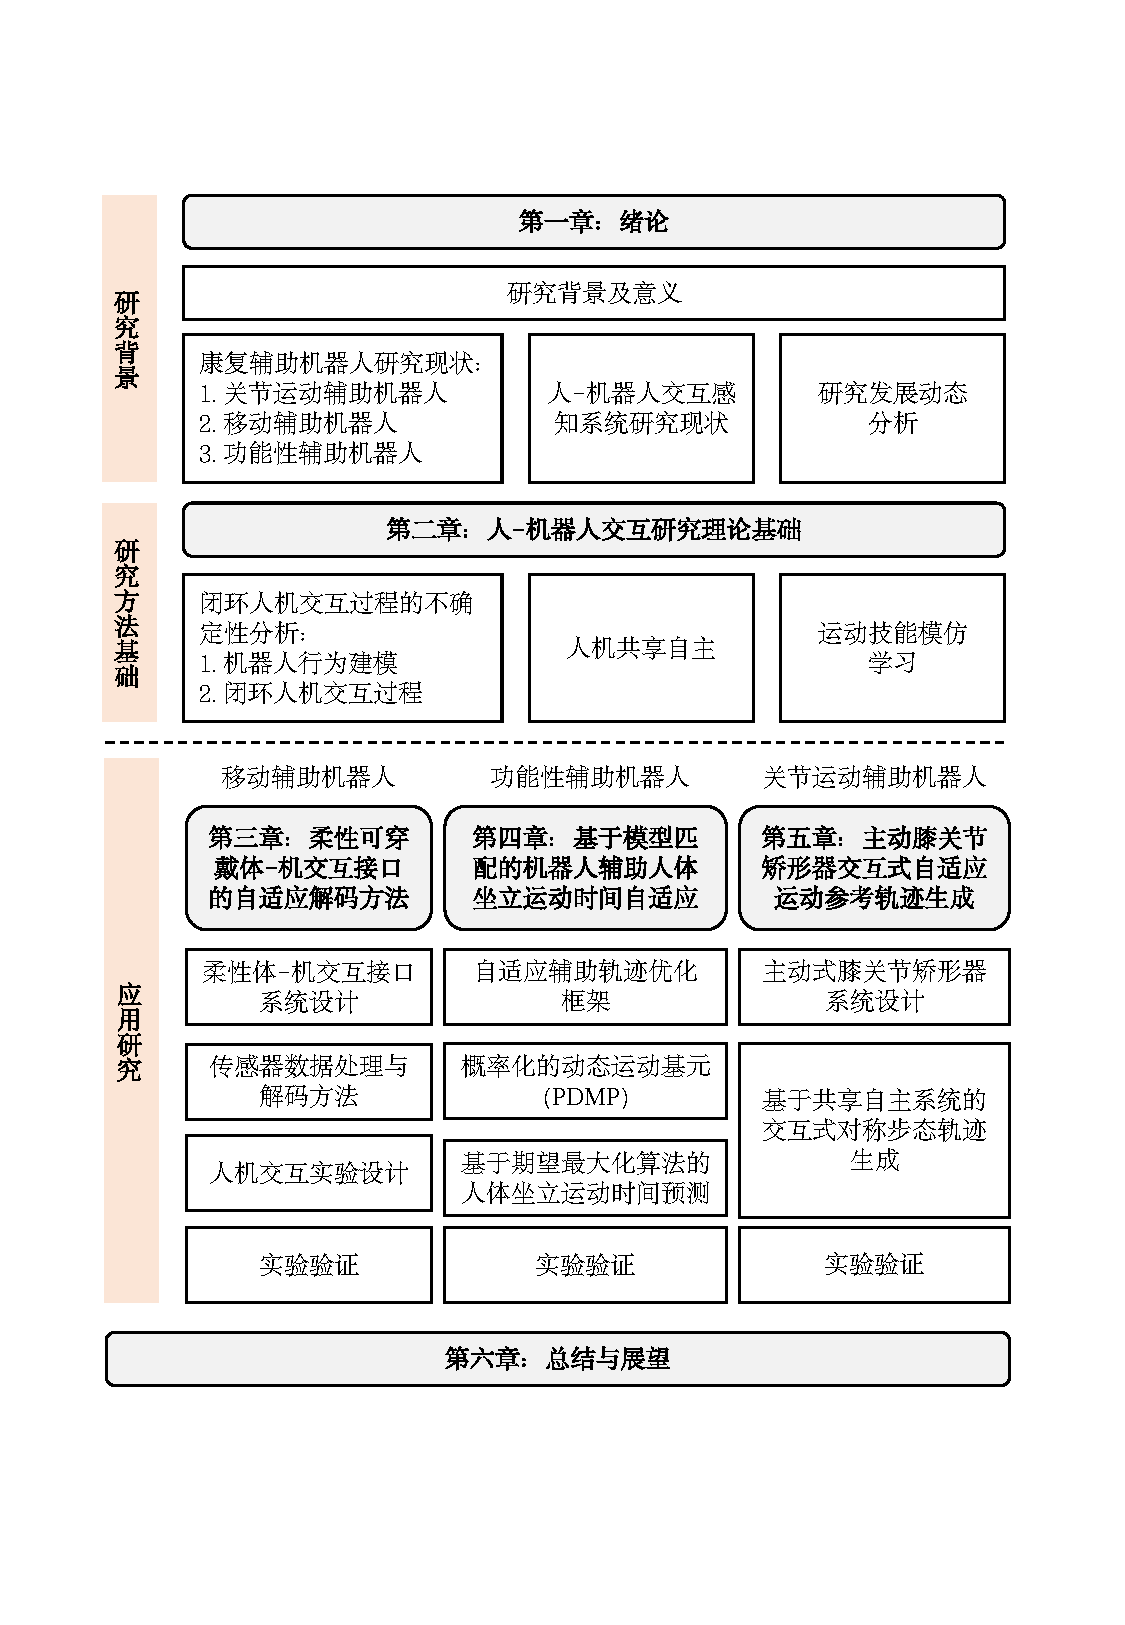
\includegraphics[width=1\textwidth]{1-Fig-6.pdf}
  \caption{部分柔性传感器在运动捕捉领域应用的研究成果}
  \label{fig:1-6}
\end{figure}

基于生理信号的辅助设备交互方法,如脑电图、眼电图(Electrooculograph, EOG)以及肌电图(Electromyography, EMG)目前被广泛地研究。作为生物体的自然反应,基于生理信号的系统不易受到个体主观意识的影响,且具有可实现超前于动作的意图推理的优势。但是该种方式主要有两个缺点:第一,因为生理电信号的信噪比低,导致可靠的信号特征难以提取,如何实时地准确地识别和解码生理信号是一个关键问题;其次,生理电信号的获取需要开发专门的硬件系统,且部分侵入性较强(例如植入式脑机接口),通常较为昂贵并且不便于携带使用\cite{blabeAssessmentBrainMachine2015a,collingerFunctionalPrioritiesAssistive2013a};目前,研究者们已经提出了一些有效的信号处理和解码方法,如特征提取\cite{phinyomarkFeatureExtractionSelection2018}、隐马尔可夫模型(Hidden Markov Model, HMM)\cite{chaurasiyaSequentialStudyEmotions2019}、支持向量机(Support Vector Machine, SVM)\cite{richhariyaEEGSignalClassification2018}等。同时,一些研究者还尝试利用深度学习技术,如卷积神经网络(Convolutional Neural Network, CNN)\cite{briouzaConvolutionalNeuralNetworkBased2021}、循环神经网络(Recurrent Neural Network, RNN)\cite{suppiahFuzzyInferenceSystem2022}、深度信念网络(Deep Belief Network, DBN)\cite{zhengEEGbasedEmotionClassification2014}以及Transformer网络\cite{montazerinTransformerbasedHandGesture2023,wanEEGformerTransformerBased2023}等方法来提高信号识别和解码的准确性,并减少数据处理所需的硬件数量,从而设计更用户友好的交互设备。

基于多模态的交互感知技术包括对语音、图像、文字、眼动、触觉以及脑电图、心电图等各类型的感知信号的综合使用\cite{suRecentAdvancementsMultimodal2023}。在数据处理上需要结合多种类型的感知手段,以协调的方式获取和处理两个或多个组合的输入信息。例如采用视觉与惯性传感器相结合的方式解决运动捕捉中视觉遮挡问题\cite{mallesonRealTimeFullBodyMotion2017,moniruzzamanWearableMotionCapture2023},提高系统鲁棒性。Riggozlio等人\cite{rizzoglioHybridBodyMachineInterface2020}结合EMG肌肉电信号和IMU运动信号设计了一种多模态身体-机器接口,并评估了其在不同融合策略下的性能。近年来,随着大语言模型技术的不断发展,也有研究尝试通过整合计算机视觉、自然语言处理、认知架构和社会信号处理等工具,来提高人-机器人的交互质量和感知的智能水平\cite{dongHuBoVLMUnifiedVisionLanguage2023,huangVoxPoserComposable3D2023,gaoPhysicallyGroundedVisionLanguage2023}。然而,多模态交互在一定程度上增加了人机交互的复杂度,用户需要理解和选择适合当前情境的交互方式,并适当地与机器人进行交互。此外,在技术层面,多模态交互涉及不同类型的数据融合,将这些不同类型的数据融合在一起是一个关键性挑战,需要在研究中进一步解决数据一致性、数据关联和数据整合等问题。

\section{研究发展动态分析}
从机器人实现的功能角度来看,针对不同的应用场景各类研究存在着差异化的结构设计以及功能实现方式。与工作在固定场景中的工业机器人等传统机器人相比,作为一种服务机器人,康复辅助机器人的一个共同的特点是需要在存在高度不确定性的非结构化环境中工作,且需要与人类进行更加丰富地交互。

随着传感器、驱动器以及相关智能算法研究的不断发展,康复辅助设备已经由传统的自动化设备逐渐向具有自主性的智能机器人发展。现阶段的辅助机器人智能化研究从``以机器为中心''逐渐向``以人为中心''过渡,不仅仅需要在功能性上满足使用者的需求,更需要与传统机器人完全不同的性能评价要求,其包括了从安全性、遵从性、舒适度、适应性、功能和灵活性等多方面的综合考虑\cite{heSurveyHumancenteredIntelligent2017b}。例如使用人在环中优化方法\cite{dingHumanintheloopOptimizationHip2018,zhangHumanintheloopOptimizationExoskeleton2017a,awadSoftRoboticExosuit2017}通过采集人类代谢能量消耗等指标动态调整机器人辅助策略以提高对不同使用者的适应性,通过在电动轮椅上安装激光雷达以及超声波传感器进行自动避障提高移动安全性\cite{fosterReflectanceFieldMap2023,parkDiscretetimeDynamicModeling2017,walterFrameworkLearningSemantic2014},在机器人设计中引入力传感器设计柔顺控制器\cite{hong-guljunWalkingSittostandSupport2011,inhokimKinematicAnalysisSittostand2011}以及设计串联弹性驱动器(Series Elastic Actuator, SEA)等新型柔性驱动结构\cite{zhongGaitSymmetryEnhancement2022}等方法降低辅助机器人系统刚性。以人为中心的人-机器人交互研究通常围绕用户来研究机器人的设计或可用性等主题,而以机器人为中心的交互则研究算法和工程创新,以提高机器人的工作性能指标。尽管现有的大量研究成果从不同的角度对辅助机器人的性能指标进行了分析和优化,综合来看,人类安全是目前康复辅助机器人交互设计的最大的问题之一\cite{tadeleSafetyDomesticRobotics2014}。作为机器人可靠性的重要指标,安全是未来发展通用型康复辅助机器人所必须保证的基本问题。通常可以使用两种不同的方法来解决人-机器人交互中的安全问题:(1)通过设计改进硬件本身或降低机器人自主性使用低水平控制策略来提高机器人的内在安全水平,这样即使发生碰撞,对人体的影响也能最小化\cite{haddadinNewInsightsConcerning2010};(2)通过设计机器人的决策规划算法让机器人的行为安全,这也被称为``交互安全''\cite{liuDesigningRobotBehavior}。

由于人-机器人交互系统是一个刚体-柔性体-软体耦合的高度复杂系统,考虑到著名的墨菲定律:``任何可能出错的事情最终都会出错'',因此在一个涉及一定风险的人-机器人交互系统中,需要充分考虑到感知、决策规划、控制执行等各个层面的不确定因素。

\begin{itemize}
\item 在交互感知方面,大多研究使用更多的传感器、开发和设计更复杂的模型以实现更高精度的状态估计或意图识别。由于不同模态的数据输入显著增加了系统的复杂度,无模型的数据驱动算法被广泛采用。由于可以在不依赖于精确建模的情况下提高系统的性能,因此无模型方法在辅助机器人状态感知、交互意图推理等方面发挥了重要的作用。然而,数据驱动方法的一个关键挑战是如何获得足够高质量的数据。其中在质量方面,数据通常来自多种传感器,这些传感器在不同情况下可能会受到噪声、遮挡、运动模糊等因素的影响,在数量上面,人机混合系统通常难以通过实物或仿真获得大量的数据,因此限制了先进与大规模算法的落地应用。此外,在辅助机器人的实际开发中,为了减少发生风险的可能,对于感知推理识别算法的可解释性和可靠性往往具有更高要求。

\item 在决策规划方面,辅助机器人交互安全面临的一个重大挑战是如何在减少机器人决策规划的保守性的同时保持对人类不确定行为变化的鲁棒性。大多数辅助和康复机器人的安全决策设计尽管在功能上能够提供所需的输出和执行预期任务,但由于通常是用降低系统的自主性的方法保证安全可靠,也没有在设计和控制概念中充分考虑人类用户的需求往往,因此效率受到质疑。近年来,以人为中心的交互决策方法考虑通过各个方面,如人类决策行为特征、神经和肌肉骨骼系统、感知系统置信度等各个方面,通过设计算法实现对用户能力的自适应成为一种新的可行方案。

\item 在控制执行层面,随着计算机设备计算能力的快速迭代发展,模型预测控制、线性二次型调节器等优化控制方法被越来越多地应用在辅助机器人当中。优化控制方法可以处理多输入多输出系统并适应外部的不确定性和干扰,通过考虑约束条件,如物理限制、关节限制以及安全性边界条件等,极大地提高了系统鲁棒性。然而,对于人机耦合的辅助机器人系统来说,在线优化的计算成本较高,实时性可能受到影响,此外对模型精度要求较高,如果模型不准确,可能导致控制效果不佳。因此,如何建立并简化人机耦合动力学模型约束以及实现高效的优化求解是目前实现优化控制方法在人机交互领域的主要挑战。
\end{itemize}

康复辅助机器人的人机交互研究包含了从传感器应用到算法设计再到本体开发的诸多内容,需要在设计时着重考虑安全性、个体适应性是其区别于其他种类机器人的典型特征。然而这两者往往是相悖的,过分强调安全排除一切可能造成风险的不确定性因素会导致机器人倾向于保守进而降低使用者体验。另一方面,人类行为虽然在许多方面明显有规则约束并且可预测,但它也始终是可变的、个体的,甚至是随机的,将更多使用者的自主行为引入交互系统中则会导致系统存在不可控的风险。因此,使用者与具有自主性的辅助机器人共同存在于一个控制系统中,即系统的控制权需要在人和机器人之间分配和协调\cite{ZhaoQianTanKongZhiZhongDeGongXiangXinXiHeGongXiangZiZhu2021}。近年来,人机共享自主的概念成为解决以上问题的一种可行途径,它主要围绕如何``理解和设计在两种各自具有一定程度自主性的实体间的交互空间''进行研究\cite{abbassTrustedAutonomyCognitive2016}。现有的共享自主框架仍然缺乏系统性和完整性,也缺乏对该领域中若干关键基础性问题的研究。在本文中,研究对人机混合闭环交互系统的结构与可能的不确定性来源进行了总结和分析,并且在此基础上进一步地对于考虑人机交互不确定性的共享自主方法应用在辅助机器人上的可能性进行了探索。

\section{研究内容及章节结构安排}
围绕康复辅助机器人中关于人机交互的共性问题,本文就如何分析和处理人机交互过程中的不确定性进行了研究。首先,本章对现有人机交互的理论基础进行了回顾与梳理,识别出其中与交互不确定性相关的关键因素。通过理论分析,研究揭示了不确定性在闭环人机交互过程中的来源及其对交互性能可能产生的影响。尽管不确定性是不可避免的,但它可以通过适当的设计和管理来最小化。通过显式地表示交互动作以及其中存在的不确定性,围绕人机共享自主的概念建立概率模型,研究实现了不同场景下的交互意图感知方法。其中涵盖了非侵入式移动辅助机器人操控、站立功能辅助机器人运动速度自适应以及步态对称性关节运动辅助机器人自适应轨迹规划等多个典型应用。图\ref{fig:1-7}给出了本文研究内容及章节结构安排结构框图,具体如下:
\begin{figure}[h]
  \centering
  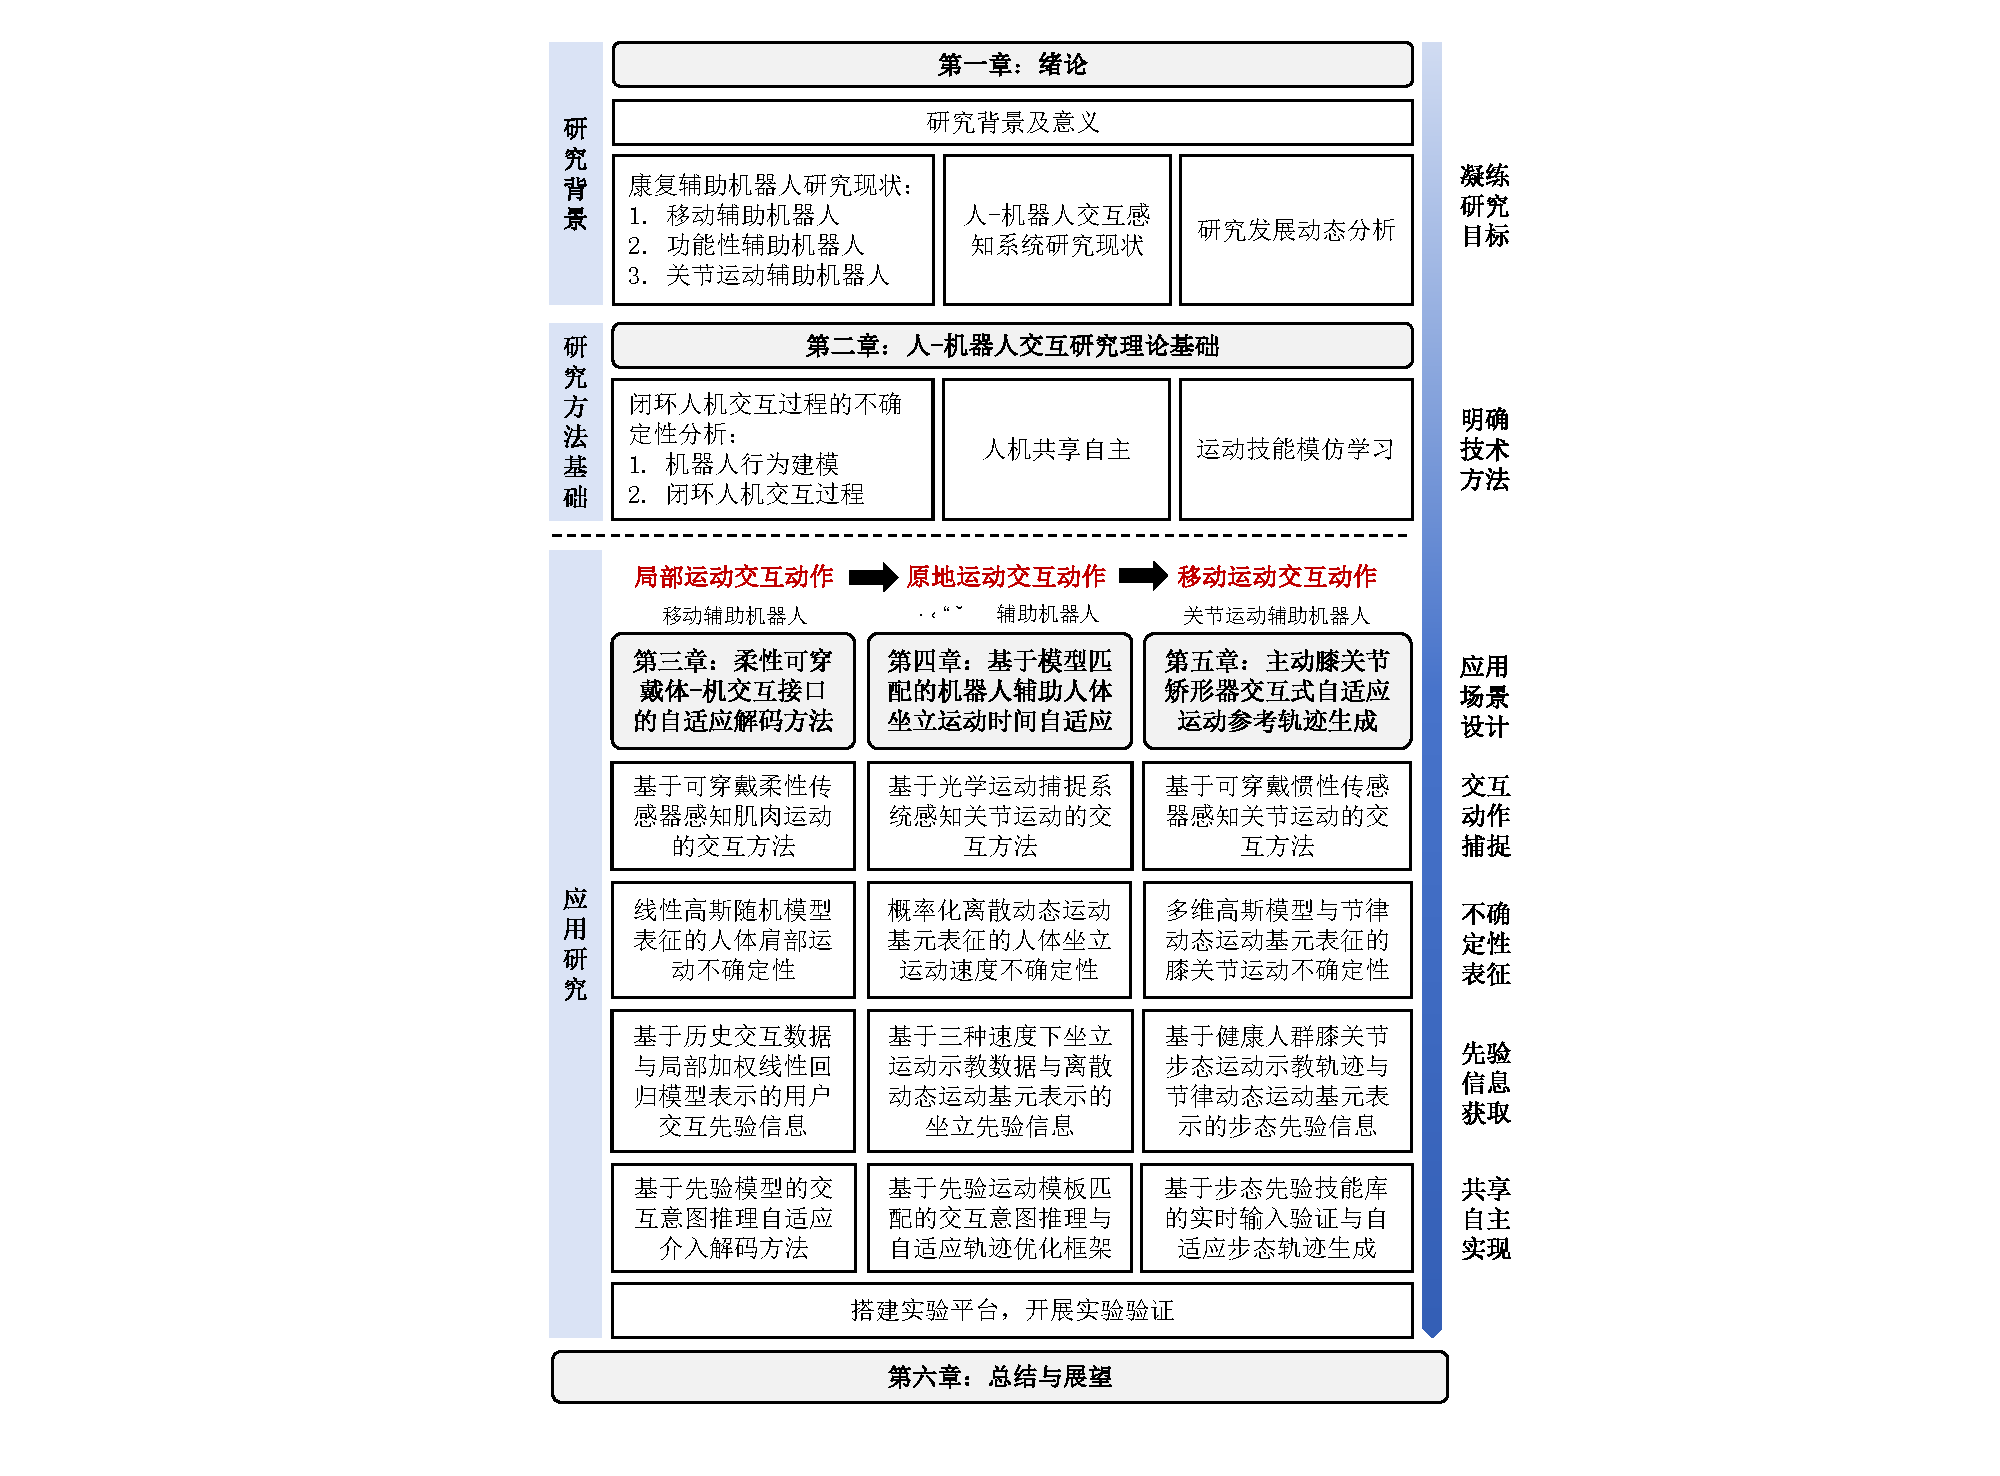
\includegraphics[width=0.93\textwidth]{1-Fig-7.pdf}
  \caption{研究内容及章节安排结构框图}
  \label{fig:1-7}
\end{figure}

第二章主要在理论层面对人机交互过程进行了分析。首先从机器人行为系统的建模过程的总结和分析出发,在此基础上从人类的视角进一步分析了闭环人机交互过程的整个流程以及其中存在的不确定性来源。此外,就处理人机交互过程中的不确定性问题,引入了共享自主的概念和相关应用方式。最后针对在共享自主方法中的人类行为表示方法,介绍了运动基元的相关理论,并就动态运动基元这一典型代表展开了详细的分析和介绍。

第三章围绕移动辅助机器人应用中新型人机交互方式展开了研究。针对局部的肩部运动交互动作,研究通过集成多组柔性弯曲拉伸传感器和一个惯性传感器设计了一种新型非侵入式可穿戴体-机交互接口,其可将残余肩部运动重新映射到二维连续命令空间以操控一个虚拟轮椅。此外,研究通过使用概率图模型对人机交互过程中的不确定性来源进行了分析,并基于此设计了一种基于规则的确定性数据映射解码方式和一种考虑到交互不确定性的意图推理数据解码方法。在此基础上,围绕一个共享自主系统,该章节中提出了一种自适应切换解码方法,它将用户的使用确定性数据映射模式操控光标的先验表现集成到一个非线性仲裁函数中,实现两种数据解码方法的自适应切换。其不仅提高了使用者操控命令生成的准确性,同时保证了数据解码方法的动态性能以适应不同任务的要求。

第四章围绕站立功能辅助机器人应用中对于被辅助对象完成站立速度的不确定性自适应问题展开了研究。针对在原地完成的坐立交互动作,研究通过离散动态运动基元对人体下肢站立运动中的踝、膝、髋关节的运动轨迹进行了表征,并对其进行概率建模。通过采集真实场景下的人体坐立离线运动数据,研究建立了一个包含快速、中速、慢速运动轨迹模板的先验技能库。为了实现根据当前部分对被辅助对象的观测实在线坐立运动时间估计,通过将该问题看做一个系统参数辨识问题,研究了基于期望最大化算法的连续人体运动时间估计方法。此外,所设计交互意图估计方法通过一个置信度水平量化指标可以嵌入一个共享自主系统中,进一步实现辅助机器人的稳定在线运动轨迹优化。

第五章围绕一个用于偏瘫患者步态对称性康复训练的主动式膝关节矫形器原型样机,介绍了一种通过学习偏瘫健侧步态特征的在线对称步态轨迹生成方法。针对连续进行的步态交互动作,该方法通过融合节律型动态运动基元与一个自适应非线性频率振荡器,实现了在线的步态运动周期轨迹的编码与解码,同时实现了下肢健侧和患侧的步态相位自适应延迟。此外,通过对健康人群的离线步行任务采集数据,设计了一个带有先验步态技能库的共享自主模块,以自适应地分析和仲裁来自未受影响侧的实时用户输入,从而最大程度地减轻输入不确定性的影响。

最后,第六章对文章研究内容进行了总结,并对当前研究存在的问题以及未来可能的研究方向进行了分析。

\section{本章小结}
本章就康复辅助机器人的研究背景及意义进行了说明。此外,通过将常见的康复辅助机器人分为移动辅助机器人、关节运动辅助机器人以及功能型辅助机器人三个大类,本章首先对它们的国内外研究现状进行了调研。就辅助机器人人机交互感知系统的研究现状进行了总结,并对用于人机交互动作测量感知各类型传感器进行了分类并分析了其优缺点。最后,我们基于对当前相关研究工作总结,对领域研究发展动态进行了分析,并分别介绍了本文各个章节的细分研究内容。
